\documentclass[10pt]{article}
\usepackage[polish]{babel}
\usepackage[utf8]{inputenc}
\usepackage[T1]{fontenc}
\usepackage{amsmath}
\usepackage{amsfonts}
\usepackage{amssymb}
\usepackage[version=4]{mhchem}
\usepackage{stmaryrd}
\usepackage{graphicx}
\usepackage[export]{adjustbox}
\graphicspath{ {./images/} }

\title{Zadania - etap I (klasy 5-7, szkoła podstawowa) }

\author{}
\date{}


\newcommand\Varangle{\mathop{{<\!\!\!\!\!\text{\small)}}\:}\nolimits}

\begin{document}
\maketitle
POLITECHNIKA GDAŃSKA

CENTRUM NAUCZANIA MATEMATYKI\\
I KSZTALCENIA NA ODLEGłOŚ́

Zadanie 1. Punkt \(P\) jest punktem przecięcia przekątnych w prostokącie \(A B C D\) o obwodzie 180 cm . Wiadomo, że odległość punktu \(P\) od boku \(B C\) jest dwa razy większa od odległości \(P\) od boku \(A B\). Oblicz pole tego prostokąta.

Zadanie 2. Dany jest kwadrat \(A B C D\) o boku 10 cm i taki punkt \(E\) leżący wewnątrz kwadratu, że \(\Varangle E A B=75^{\circ} \mathrm{i} \Varangle A B E=30^{\circ}\). Ile wynosi pole trójkąta \(B C E\) ?

Zadanie 3. Prostokątną działkę, o powierzchni \(120 \mathrm{~m}^{2}\) podzielono na prostokątne grządki tak, jak na rysunku niżej. Niektóre wymiary są podane na rysunku. Ile wynosi powierzchnia przeznaczona pod uprawę warzyw, jeżeli grządka przeznaczona na kwiaty ma pole powierzchni równe \(40 m^{2}\) ?\\
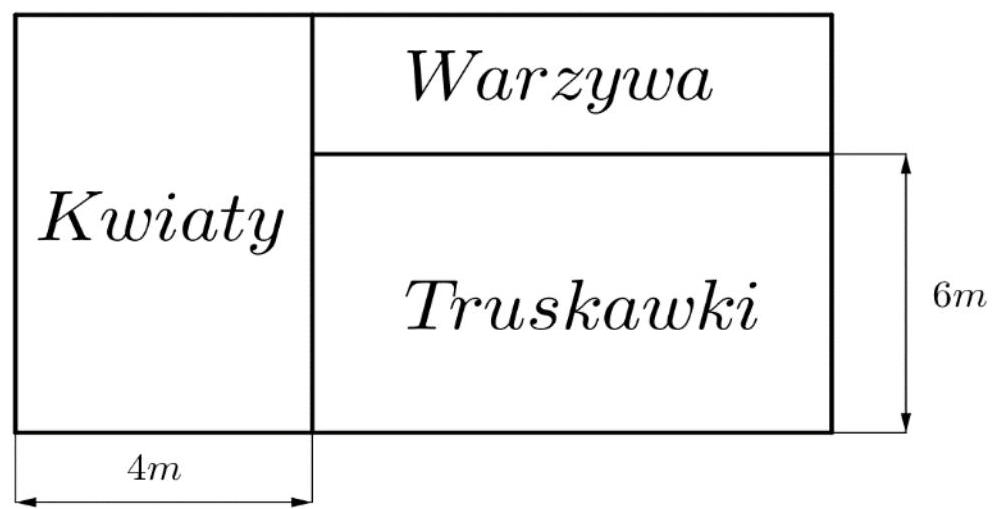
\includegraphics[max width=\textwidth, center]{2024_11_21_0e326beee08d88391e6fg-1}

Zadanie 4. W graniastosłupie prawidłowym czworokątnym krawędź podstawy jest równa 6 cm , a wysokość stanowi 250\% długości tej krawędzi. O ile procent należy zwiększyć długość krawędzi podstawy tego graniastosłupa, żeby suma długości wszystkich krawędzi graniastosłupa była równa 144 cm ?

Zadanie 5. Znajdź takie cyfry \(A, B\) i \(C\), żeby \(A B+B A=C A C(A B, B A\) oznaczają liczby dwucyfrowe, natomiast \(C A C\) liczbę trzycyfrową).\\
imię i nazwisko uczestnika

CENTRUM NAUCZANIA MATEMATYKI\\
I KSZTALCENIA NA ODLEGLOŚ\\
\(\qquad\)

\section*{ZAŁACZNIK DO KARTY UCZESTNIKA KONKURSU „OD SZKOLNIAKA DO ŻAKA"}
\section*{Oświadczenie}
Niniejszym oświadczam, że jako uczestnik konkursu „Od szkolniaka do żaka" zorganizowanego przez Centrum Nauczania Matematyki i Kształcenia na Odległość Politechniki Gdańskiej, wyrażam zgodę na przetwarzanie moich danych osobowych w zakresie niezbędnym dla potrzeb niniejszego konkursu.

Przyjmuję do wiadomości, że moje dane osobowe będą wykorzystane zgodnie z ustawą z dnia 29 sierpnia 1997 r. o ochronie danych osobowych (Dz.U. 1997 nr 133 poz. 883) dla celów przeprowadzenia w/w konkursu.

Jednocześnie oświadczam, że zostałem poinformowany o tym, że:

\begin{itemize}
  \item Administratorem danych osobowych konkursu jest: Politechnika Gdańska z siedzibą przy ul. Gabriela Narutowicza 11/12; 80-233 Gdańsk
  \item Przysługuje mi prawo do wglądu do moich danych i żądania ich poprawienia.
  \item Dane będą przetwarzane dla realizacji konkursu.
  \item Podanie danych jest dobrowolne.
  \item Nie przewiduje się przekazywania danych.
\end{itemize}

Wyrażam zgodę na uczestnictwo mojego dziecka w konkursie „Od szkolniaka do żaka"

Data \(\qquad\) r.\\
(podpis rodzica lub opiekuna prawnego ucznia)

Akceptuję i wyrażam zgodę na postanowienia regulaminu konkursu „Od szkolniaka do żaka" zamieszczonego na stronie internetowej konkursu: http:Ilpg.edu.pl/ kursyzmatematyki/o-konkursie

Data \(\qquad\) r.


\end{document}